%%%%%%%%%%%%%%%%%%%%%%%%%%%%%%%%%%%%%%%%%%%%%%%%%%%%%%%%%%%%%%%%%%%%%%%%%%%%%%
%%% 				Customizações do abnTeX2 para o IFCE    			   %%%
%%% 		Instituto Federal de Educação, Ciência e Tecnologia do Ceará   %%%
%%% Template disponível em: https://github.com/clodomirneto/IFCETeX2	   %%%
%%% Desenvolvedores do IFCETeX2: Professor Clodomir Silva Lima Neto	       %%%
%%% 							 Professor Marcelo Araújo Lima		       %%%
%%% 					  	     Professor Antonio Sergio de Sousa Vieira  %%%
%%% E-mails para contato: clodomir.neto@ifce.edu.br						   %%%
%%% 					  marcelo.alima@ifce.edu.br					       %%%
%%% 					  sergio.vieira@ifce.edu.br					       %%%
%%%%%%%%%%%%%%%%%%%%%%%%%%%%%%%%%%%%%%%%%%%%%%%%%%%%%%%%%%%%%%%%%%%%%%%%%%%%%%

%%%%%%%%%%%%%%%%%%%%%%%%%%%%%%%%%%%%%%%%%%%%%%%%%%%%%%%%%%%%%%%%%%%%%%%%%%%%%%
%%% 			Instruções para Uso do Template IFCETeX2	  			   %%%
%%%																	       %%%
%%% 1. Criar uma conta no Overleaf.									       %%%
%%% 2. No Ambiente Overleaf, clicar em Menu (canto superior esquerdo) 	   %%% 
%%% 3. Clicar em "Copiar Projeto".  									   %%%
%%% 4. Dê um novo nome para o Projeto. 								       %%%
%%%%%%%%%%%%%%%%%%%%%%%%%%%%%%%%%%%%%%%%%%%%%%%%%%%%%%%%%%%%%%%%%%%%%%%%%%%%%%

%%%%%%%%%%%%%%%%%%%%%%%%%%%%%%%%%%%%%%%%%%%%%%%%%%%%%%%%%%%%%%%%%%%%%%%%%%%%%%%
%%% 				Customizações do abnTeX2 para o IFCE    			    %%%
%%% 		Instituto Federal de Educação, Ciência e Tecnologia do Ceará    %%%
%%% Template disponível em: https://github.com/clodomirneto/IFCETeX2	    %%%
%%% Desenvolvedores do IFCETeX2: Professor Clodomir Silva Lima Neto		    %%%
%%% 							 Professor Marcelo Araújo Lima              %%%
%%%                              Professor Antonio Sergio de Sousa Vieira	%%%
%%% E-mails para contato: clodomir.neto@ifce.edu.br						    %%%
%%% 					  marcelo.alima@ifce.edu.br                         %%%
%%%                       sergio.vieira@ifce.edu.br	                        %%%
%%%%%%%%%%%%%%%%%%%%%%%%%%%%%%%%%%%%%%%%%%%%%%%%%%%%%%%%%%%%%%%%%%%%%%%%%%%%%%%

\documentclass[        
    a4paper,          % Tamanho da folha A4
    12pt,             % Tamanho da fonte 12pt
    chapter=TITLE,    % Todos os capitulos devem ter caixa alta
    %section=TITLE,   % Todas as secoes devem ter caixa alta
    oneside,          % Usada para impressao em apenas uma face do papel
    english,          % Hifenizacoes em ingles
    spanish,          % Hifenizacoes em espanhol
    brazil            % Ultimo idioma eh o idioma padrao do documento
]{abntex2}

% Importações de pacotes
\usepackage[utf8]{inputenc}                         % Acentuação direta
\usepackage[T1]{fontenc}                            % Codificação da fonte em 8 bits
\usepackage{graphicx}                               % Inserir figuras
\usepackage{amsfonts,amssymb,amsmath}               % Fonte e símbolos matemáticos
\usepackage{booktabs}                               % Comandos para tabelas
\usepackage{verbatim}                               % Texto é interpretado como escrito no documento
\usepackage{multirow,array}                         % Múltiplas linhas e colunas em tabelas
\usepackage{indentfirst}                            % Endenta o primeiro parágrafo de cada seção.
\usepackage{listings}                               % Utilizar codigo fonte no documento
\usepackage{xcolor}
\usepackage{microtype}                              % Para melhorias de justificação?
\usepackage[portuguese,ruled,lined]{algorithm2e}    % Escrever algoritmos
\usepackage{algorithmic}                            % Criar Algoritmos  
%\usepackage{float}                                 % Utilizado para criação de floats
\usepackage{amsgen}
\usepackage{lipsum}                                 % Usar a simulação de texto Lorem Ipsum
%\usepackage{titlesec}                               % Permite alterar os títulos do documento
\usepackage{tocloft}                                % Permite alterar a formatação do Sumário
\usepackage{etoolbox}                               % Usado para alterar a fonte da Section no Sumário
%\usepackage[nogroupskip,nonumberlist,acronym]{glossaries}                % Permite fazer o glossario
\usepackage{caption}                                % Altera o comportamento da tag caption
\usepackage[alf,abnt-emphasize=bf,bibjustif, recuo=0cm,abnt-etal-cite=3,abnt-etal-list=0,abnt-etal-text=it]{abntex2cite}  % Citações padrão ABNT
%\usepackage[bottom]{footmisc}                      % Mantém as notas de rodapé sempre na mesma posição
%\usepackage{times}                                 % Usa a fonte Times
\usepackage{mathptmx}                               % Usa a fonte Times New Roman							
%\usepackage{lmodern}                               % Usa a fonte Latin Modern
%\usepackage{subfig}                                % Posicionamento de figuras
%\usepackage{scalefnt}                              % Permite redimensionar tamanho da fonte
%\usepackage{color, colortbl}                       % Comandos de cores
%\usepackage{lscape}                                % Permite páginas em modo "paisagem"
%\usepackage{ae, aecompl}                           % Fontes de alta qualidade
%\usepackage{picinpar}                              % Dispor imagens em parágrafos
%\usepackage{latexsym}                              % Símbolos matemáticos
%\usepackage{upgreek}                               % Fonte letras gregas
\usepackage{appendix}                               % Gerar o apendice no final do documento
\usepackage{paracol}                                % Criar paragrafos sem identacao
\usepackage{ifcetex2}		                        % Biblioteca com as normas do IFCE para trabalhos academicos
\usepackage{pdfpages}                               % Incluir pdf no documento
\usepackage{textcomp}
% Organiza e gera a lista de abreviaturas, simbolos e glossario
%\makeglossaries
% Gera o Indice do documento
%\makeindex

%TEOREMAS

\newtheorem{proposition}{Proposição}[chapter]
\newtheorem{theorem}{Teorema}[chapter]
\newtheorem{lemma}{Lema}[chapter]
\newtheorem{definition}{Definição}[chapter]
\newtheorem{exemplo}{Exemplo}[chapter]
\newtheorem{corollary}{Corolário}[chapter]
\newtheorem{exercicio}{Exercício}[chapter]

%PROVAS

\newenvironment{prova}[1][Prova]{\noindent\textbf{#1.} }{\hfill\rule{0.5em}{0.5em}}
\newenvironment{dem}[1][Demonstra\c c\~ao]{\noindent\textbf{#1.} }{\hfill\rule{0.5em}{0.5em}}
\newenvironment{exm}{\noindent{\textbf{Exemplo:}}}{}

% Opções disponíveis

%\trabalhoacademico{tese}
%\trabalhoacademico{dissertacao}
%\trabalhoacademico{tccespecializacao}
\trabalhoacademico{tccgraduacao}

% Define se o trabalho é uma qualificação, coloque 'nao' para versão final do trabalho

\ehqualificacao{nao}

% Remove as bordas vermelhas e verdes do PDF gerado, coloque 'sim' para remover

\removerbordasdohyperlink{sim} 

% Adiciona a cor azul a todos os hyperlinks

\cordohyperlink{nao}

% Informação relacionadas ao trabalho

\autor{João Pedro Moreira Campos de Lima\\Isaac da Cunha Cavalcanti Duarte\\Juliano Magalhães Jurity}
\titulo{Raciocínio Lógico em LLMs: Análise de Processos Dedutivos na Resolução de Sudoku}
\local{Maracanaú}
\data{2026}

% Informação sobre a IES

\ies{Instituto Federal de Educação, Ciência e Tecnologia do Ceará}
\iessigla{IFCE}
\centro{\textit{Campus} Maracanaú}

% Informação para Tese

\programadoutorado{Programa de Pós-Graduação em Saúde Coletiva}
\nomedodoutorado{Doutorado em Saúde Coletiva}
\doutorem{Saúde Coletiva}
\areadeconcentracaodoutorado{Saúde Coletiva}

% Informação para Dissertacao

\programamestrado{Programa de Pós-Graduação em Ciência da Computação}
\nomedomestrado{Mestrado Acadêmico em Ciência da Computação}
\mestreem{Ciência da Computação}
\areadeconcentracaomestrado{Ciência da Computação}

% Informação para TCC de Especialização

\especializacaoem{Ensino de Ciências da Natureza e Matemática}
\habilitacaoesp{Especialista}
\areadeconcentracaoespecializacao{Ensino de Matemática}

% Informação para TCC de Graduação

\graduacaoem{Ciência da Computação}
\habilitacao{Bacharel}
\areadeconcentracaograduacao{Ciência da Computação}

% Data de Aprovação

\dataaprovacao{\underline{\hspace*{1cm}}/\underline{\hspace*{1cm}}/\underline{\hspace*{1.2cm}}.}

% Abreviaturas dos títulos acadêmicos

% Especialista: Esp.
% Mestre: Me.
% Mestra: Ma.
% Doutor: Dr.
% Doutora: Dra.

% Informação sobre o Orientador

\orientador{Profa. Aurenivia Ferreira da Silva}
\orientadories{Instituto Federal de Educação, Ciência e Tecnologia do Ceará}
\orientadoriessigla{IFCE}
\orientadorcentro{\textit{Campus} Caucaia}
\orientadorfeminino{sim} % Coloque 'sim' se for do sexo feminino

% Informação sobre o Coorientador

\coorientador{} % Deixe o nome do coorientador em branco para remover do documento
\coorientadories{Instituto Federal de Educação, Ciência e Tecnologia do Ceará}
\coorientadoriessigla{IFCE}
\coorientadorcentro{\textit{Campus} Caucaia}
\coorientadorfeminino{sim} % Coloque 'sim' se for do sexo feminino

% Folha de rosto adaptada para o trabalho da disciplina.
\makeatletter
\renewcommand{\folhaderostocontent}{%
  \begin{center}
    \normalsize\MakeUppercase\imprimirautor\par
    \vspace{2cm}
    \normalsize\MakeUppercase\imprimirtitulo\par
  \end{center}
  \vspace{1.5cm}
  \hspace*{8cm}%
  \begin{minipage}{8cm}
    \begin{SingleSpace}
      Projeto de Pesquisa apresentado ao Curso de Ciência da Computação do Instituto Federal de Educação, Ciência e Tecnologia do Ceará -- IFCE \textit{Campus} Maracanaú, como requisito parcial para aprovação na disciplina de Metodologia Científica.

      \vspace{\onelineskip}
      Orientadora: Profa. Ma. Aurenívia Ferreira da Silva.
    \end{SingleSpace}
  \end{minipage}
  \vfill
  \centering
  \normalsize\MakeUppercase\imprimirlocal\par
  \normalsize\MakeUppercase\imprimirdata
}
\makeatother

% Seções primárias sem quebra obrigatória de página, conforme o modelo da disciplina.
\newcommand{\secaoprimariasemquebra}[1]{%
  \refstepcounter{chapter}%
  \section*{\thechapter\quad\MakeUppercase{#1}}%
  \addcontentsline{toc}{chapter}{\thechapter\quad\MakeUppercase{#1}}%
}

% Informação sobre a banca

% Membro da Banca Dois

\membrodabancadois{Prof. Dra. XXXXX}
\membrodabancadoisies{Instituto Federal de Educação, Ciência e Tecnologia do Ceará}
\membrodabancadoisiessigla{IFCE}
\membrodabancadoiscentro{\textit{Campus} Caucaia}

% Membro da Banca Três

\membrodabancatres{Prof. Dra. XXXXX}
\membrodabancatresies{Instituto Federal de Educação, Ciência e Tecnologia do Ceará}
\membrodabancatresiessigla{IFCE}
\membrodabancatrescentro{\textit{Campus} Caucaia}

% Informação Complementar sobre a banca

\membrodabancaquatro{Membro da Banca Quatro}
\membrodabancaquatrocentro{Centro de Ciências e Tecnologia - CCT}
\membrodabancaquatroies{Universidade do Membro da Banca Quatro - SIGLA}
\membrodabancacinco{Membro da Banca Cinco}
\membrodabancacincocentro{Teste}
\membrodabancacincoies{Universidade do Membro da Banca Cinco - SIGLA}
\membrodabancaseis{Membro da Banca Seis}
\membrodabancaseiscentro{}
\membrodabancaseisies{Universidade do Membro da Banca Seis - SIGLA}

\begin{document}	

% Elementos pré-textuais

\imprimircapa
\imprimirfolhaderosto{}
%\imprimirfichacatalografica{elementos-pre-textuais/ficha-catalografica}
%\imprimirerrata{elementos-pre-textuais/errata}
%\imprimirfolhadeaprovacao
%\imprimirdedicatoria{elementos-pre-textuais/dedicatoria}
%\imprimiragradecimentos{elementos-pre-textuais/agradecimentos}
%\imprimirepigrafe{elementos-pre-textuais/epigrafe}
%\imprimirresumo{elementos-pre-textuais/resumo}
%\imprimirabstract{elementos-pre-textuais/abstract}
%\imprimirlistadefiguras
%\imprimirlistadetabelas
%\imprimirlistadequadros
%\imprimirlistadealgoritmos
%\imprimirlistadecodigosfonte
%\imprimirlistadesiglas{elementos-pre-textuais/lista-de-siglas}
%\imprimirlistadesimbolos{elementos-pre-textuais/lista-de-simbolos}
\imprimirsumario
	
% Elementos textuais

\textual
\chapter{Introdução}

\section{Delimitação do tema}

Modelos de Linguagem de Grande Escala, ou LLMs, são sistemas capazes de ler e produzir textos. Eles costumam responder de forma fluida e convincente, mas uma explicação bem escrita não garante que o raciocínio apresentado esteja correto. Esta pesquisa investiga essa diferença em uma tarefa simples de conferir: encontrar e explicar uma única jogada de Sudoku.

O Sudoku foi escolhido porque suas regras são objetivas. Uma pessoa ou um programa pode verificar se uma jogada respeita a linha, a coluna e o bloco da célula. Isso permite observar duas coisas separadamente: se a LLM chegou ao valor certo e se a explicação que ela deu realmente justifica esse valor.

O estudo trabalha com Sudokus 4 $\times$ 4 e 9 $\times$ 9. O tabuleiro começa com algumas células preenchidas, chamadas pistas, e outras vazias. O objetivo é preencher as células vazias sem alterar as pistas. Em cada linha, coluna e bloco, cada número permitido deve aparecer uma única vez. No Sudoku 4 $\times$ 4, usam-se os números de 1 a 4 e os blocos têm 2 $\times$ 2 células. No Sudoku 9 $\times$ 9, usam-se os números de 1 a 9 e os blocos têm 3 $\times$ 3 células.

\begin{figure}[!ht]
\centering
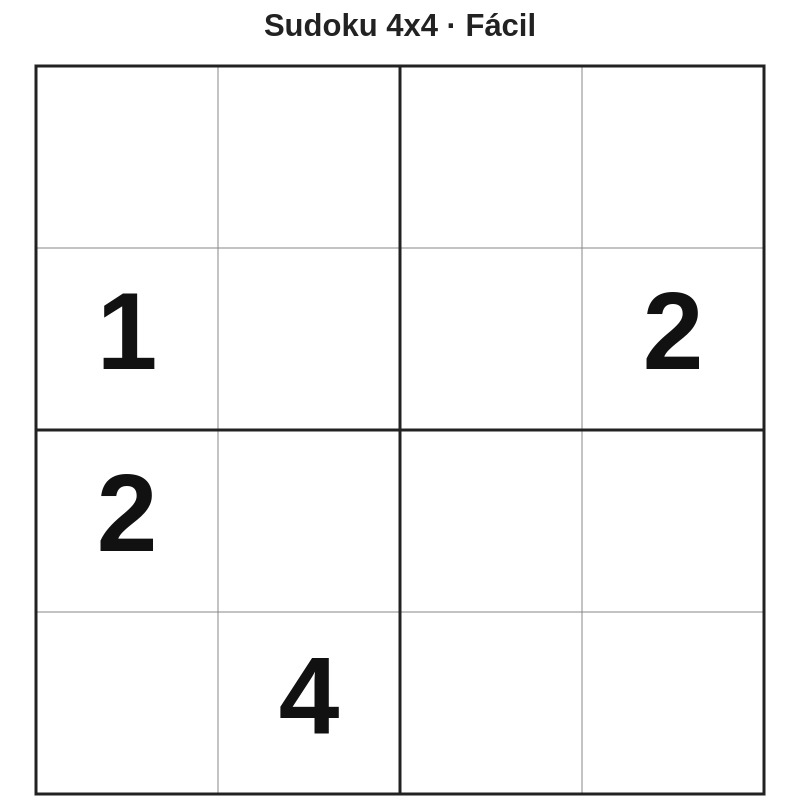
\includegraphics[width=0.62\textwidth]{figuras/sudoku-4x4-easy}
\Caption{Exemplo de tabuleiro Sudoku 4 $\times$ 4\label{fig:intro-sudoku}}
\Fonte{EducColorir (s.d.). Disponível em: \url{https://www.educolorir.com/gerador-de-sudoku}. Acesso em: 21 out. 2026.}
\end{figure}

Para indicar uma posição, o texto usa a forma L$\mathit{x}$C$\mathit{y}$, em que L significa linha e C significa coluna. A contagem começa em 1. Assim, L1C4 é a célula da primeira linha e da quarta coluna. Essa é uma notação pensada para leitura humana; mais adiante, a metodologia mostra como a mesma posição aparece no programa.

Uma célula vazia pode receber apenas números que não estejam em sua linha, coluna ou bloco. Esses números possíveis são chamados de candidatos. Se, em um Sudoku 4 $\times$ 4, uma célula não pode receber 1, 2 ou 4, resta apenas o número 3. A partir dessa ideia, a pesquisa analisa três maneiras de encontrar uma jogada.

No \textit{Naked Single}, uma célula fica com apenas um candidato. No \textit{Hidden Single}, um número pode continuar sendo candidato em mais de uma célula do tabuleiro, mas só pode aparecer em uma posição de uma linha, coluna ou bloco. No consenso de primeira camada, o programa considera hipóteses temporárias, acompanha o que acontece em cada uma e procura uma conclusão que se repete em todos os caminhos possíveis.

O recorte do estudo é uma jogada por vez e somente essas três técnicas. A intenção não é afirmar como uma LLM funciona internamente. O objetivo é verificar se ela produz uma jogada válida e se a explicação apresentada combina com a técnica solicitada.

\section{Problematização}

Quando uma LLM apresenta uma resposta convincente, é fácil assumir que ela raciocinou corretamente. Em tarefas lógicas, porém, ela pode acertar o valor por outro caminho, usar uma técnica diferente da pedida ou escrever uma justificativa que não sustenta a conclusão. Avaliar apenas a resposta final deixa esses casos escondidos.

O Sudoku cria um ambiente controlado para observar esse problema. As regras são claras, a jogada pode ser conferida automaticamente e a dificuldade pode ser ajustada. As técnicas de \textit{Naked Single} e \textit{Hidden Single} dependem apenas das informações visíveis no tabuleiro. O consenso exige que a LLM acompanhe hipóteses e compare as consequências de cada uma.

Diante disso, a pesquisa busca responder: como as LLMs se comportam ao indicar e justificar uma jogada de Sudoku que exige uma dedução direta ou uma comparação entre hipóteses?

\section{Hipótese}

Espera-se que as LLMs tenham melhor desempenho em \textit{Naked Single} e \textit{Hidden Single}, pois essas técnicas dependem de restrições visíveis na grade. No consenso, espera-se mais dificuldade, porque a tarefa exige manter hipóteses temporárias, acompanhar suas consequências e encontrar uma conclusão comum.

\section{Justificativa}

Avaliar LLMs com Sudoku ajuda a separar duas coisas que frequentemente aparecem misturadas: acertar uma resposta e explicar bem por que ela está certa. Como cada jogada pode ser conferida por regras objetivas, o estudo permite identificar respostas corretas com justificativas fracas, justificativas coerentes que chegam a uma conclusão errada e respostas que seguem exatamente a técnica solicitada.

Os resultados podem contribuir para avaliações de sistemas que precisam explicar suas decisões em linguagem clara. O estudo também oferece um conjunto de critérios simples para examinar respostas de LLMs em tarefas estruturadas, nas quais é possível conferir tanto o resultado quanto o caminho usado para chegar a ele.

\secaoprimariasemquebra{Objetivos}

\section{Objetivo geral}

\begin{alineascomponto}
\item avaliar o desempenho de LLMs na resolução e na justificativa de jogadas de Sudoku 4 $\times$ 4 e 9 $\times$ 9 que exijam deduções diretas ou raciocínio por hipóteses.
\end{alineascomponto}

\section{Objetivos específicos}

\begin{alineascomponto}
\item construir e validar um conjunto balanceado de instâncias de Sudoku classificadas segundo a aplicabilidade de \textit{Naked Single}, \textit{Hidden Single} e do princípio do consenso;
\item submeter as mesmas instâncias a LLMs selecionadas, sob comandos e configurações padronizados;
\item verificar a correção das jogadas e a adequação das justificativas, comparando o desempenho dos modelos entre deduções diretas e raciocínios por hipóteses.
\end{alineascomponto}

%\input{elementos-textuais/trabalhos-relacionados}
\secaoprimariasemquebra{Metodologia}

Esta pesquisa segue uma sequência simples. Primeiro, o programa cria tabuleiros e identifica a técnica presente em cada um. Depois, uma LLM recebe esses tabuleiros e propõe uma jogada. Por fim, o programa confere a jogada e a explicação. A implementação de referência está disponível em repositório público\footnote{Disponível em: \url{https://github.com/nayetdet/sudoku-llm-reasoning}. Acesso em: 21 out. 2026.}. O banco já existente será tratado como uma base piloto, usada para testar o processo e orientar a etapa comparativa da pesquisa.

O experimento usa Sudokus 4 $\times$ 4 e 9 $\times$ 9. Dentro do programa, uma célula vazia é representada por zero. Os demais números são as pistas do tabuleiro. Por exemplo, a posição que o leitor vê como L1C4 aparece no programa como $[0,3]$: o programa começa a contar linhas e colunas em zero, enquanto o texto começa em 1.

\section{Como o programa lê o tabuleiro}

O tabuleiro é guardado como uma matriz, isto é, uma lista de linhas. Em um Sudoku 4 $\times$ 4, há quatro linhas, quatro colunas e blocos de 2 $\times$ 2 células. Em um Sudoku 9 $\times$ 9, há nove linhas, nove colunas e blocos de 3 $\times$ 3 células.

Para cada célula vazia, o programa começa com todos os números permitidos. Em seguida, remove os números que já aparecem na linha, na coluna e no bloco da célula. Os números restantes formam o conjunto de candidatos. É a partir desse conjunto que o programa reconhece as técnicas usadas no estudo.

Em termos formais, se $x$ é uma célula vazia e $V_n=\{1,2,\ldots,n\}$ é o conjunto de números permitidos, os candidatos são calculados por:

\[
\operatorname{Cand}_G(x)=V_n\setminus\bigl(L(x)\cup C(x)\cup B(x)\bigr).
\]

Na fórmula, $L(x)$ reúne os números presentes na linha de $x$, $C(x)$ os números da coluna e $B(x)$ os números do bloco. O símbolo $\setminus$ significa ``retirar do conjunto''. A fórmula, portanto, diz exatamente o que foi explicado no parágrafo anterior: começar com todos os números e excluir os que já não podem ser usados.

O \textit{Naked Single} aparece quando a célula fica com um único candidato:

\[
\left|\operatorname{Cand}_G(x)\right|=1.
\]

O \textit{Hidden Single} aparece quando um número $v$ só pode ser colocado em uma célula de uma unidade $U$, sendo $U$ uma linha, coluna ou bloco:

\[
\left|\left\{x\in U : v\in\operatorname{Cand}_G(x)\right\}\right|=1.
\]

Para o consenso de primeira camada, o programa escolhe um número que tem mais de uma posição possível em uma mesma unidade. Cada possibilidade cria um ramo, ou seja, uma cópia temporária do tabuleiro. Dentro de cada ramo, o programa aplica apenas \textit{Naked Singles} e \textit{Hidden Singles}. Se todos os ramos viáveis chegam ao mesmo valor para uma célula alvo, esse valor é aceito no tabuleiro original. Em linguagem lógica, se $D(G_p)(t)=a$ em todos os ramos viáveis $p$, então a célula alvo $t$ recebe $a$:

\[
\forall p\in P_v^{\mathrm{viaveis}},\quad D(G_p)(t)=a
\quad\Longrightarrow\quad t=a.
\]

Aqui, $P_v^{\mathrm{viaveis}}$ representa as posições que ainda são possíveis para o valor $v$. A expressão $D(G_p)$ representa a grade depois das deduções diretas feitas no ramo $p$. A expressão ``primeira camada'' quer dizer que o programa não cria uma nova hipótese dentro do ramo: ele apenas acompanha as consequências da hipótese inicial.

\section{Como o Z3 verifica as grades}

Além de calcular candidatos, o programa usa o Z3, um solucionador de restrições lógicas. Para o Z3, cada célula é uma variável inteira entre 1 e $n$. Ele recebe três regras: os valores de uma linha não podem se repetir, os valores de uma coluna não podem se repetir e os valores de um bloco não podem se repetir. As pistas já existentes também ficam fixadas aos seus valores.

A formalização a seguir apenas escreve essas mesmas regras em símbolos. Ela acompanha diretamente o que o código entrega ao Z3: primeiro as regras da grade, depois as pistas e, por fim, a busca pelas soluções possíveis.

\subsection{Modelo lógico usado pelo Z3}

Para tornar essa etapa precisa, seja $x_{ij}$ a variável criada para a célula da linha $i$ e da coluna $j$. O código cria uma variável para cada célula, inclusive para as pistas. Em uma grade de ordem $n$, as restrições de domínio são:

\[
1 \leq x_{ij} \leq n,
\qquad 0 \leq i,j < n.
\]

Em seguida, o Z3 recebe uma restrição de valores distintos para cada linha, cada coluna e cada bloco. Se $q=\sqrt{n}$ é o tamanho do lado de um bloco, essa parte do modelo pode ser escrita como:

\[
\begin{aligned}
&\operatorname{Distinct}(x_{i0},x_{i1},\ldots,x_{i,n-1}) && \text{para toda linha } i;\\
&\operatorname{Distinct}(x_{0j},x_{1j},\ldots,x_{n-1,j}) && \text{para toda coluna } j;\\
&\operatorname{Distinct}\bigl(\{x_{rq+a,\,sq+b}:0\leq a,b<q\}\bigr) && \text{para cada bloco } (r,s).
\end{aligned}
\]

A última linha representa os blocos: $r$ e $s$ indicam em qual bloco a célula está, enquanto $a$ e $b$ indicam sua posição dentro dele. Por exemplo, em um Sudoku 9 $\times$ 9, $q=3$; cada bloco tem três linhas e três colunas. O termo \textit{Distinct} significa apenas que os valores listados devem ser diferentes entre si.

Se a entrada do tabuleiro possui uma pista $g_{ij}$ diferente de zero, o código fixa a variável correspondente:

\[
g_{ij}\neq 0 \quad \Longrightarrow \quad x_{ij}=g_{ij}.
\]

O conjunto formado por todas essas restrições será chamado de $\Phi_G$. Uma solução do Sudoku é qualquer preenchimento que respeita $\Phi_G$. Para uma posição, o programa reúne os valores que aparecem nessa posição ao percorrer todas as soluções encontradas. Se aparece apenas um valor, a posição é globalmente forçada; se aparecem dois ou mais valores, a posição continua admitindo mais de uma possibilidade. Essa noção é usada pelo código ao preencher os campos de validação da resposta da LLM. A escrita formal desse conjunto está no Apêndice A.

O Z3 procura um preenchimento completo que respeite todas essas regras. Quando encontra uma solução, o programa adiciona uma nova regra que obriga a próxima solução a ser diferente dela em pelo menos uma célula. Repetindo esse procedimento, o programa descobre se a grade não tem solução, tem uma única solução ou admite mais de uma solução.

Mais exatamente, se $M_k$ é a $k$-ésima solução encontrada, o código adiciona a restrição de bloqueio:

\[
\beta_k=\bigvee_{0\leq i,j<n}\bigl(x_{ij}\neq M_k(x_{ij})\bigr).
\]

Essa expressão obriga a próxima solução a discordar de $M_k$ em pelo menos uma célula. Depois de encontrar $k$ soluções, o Z3 procura uma nova solução para $\Phi_G\land\beta_1\land\cdots\land\beta_k$. O símbolo $\land$ significa ``e'': o Z3 precisa respeitar as regras do Sudoku e todas as restrições de bloqueio já criadas. Quando essa busca se torna insatisfatível, todas as soluções da grade foram enumeradas.

Essa etapa não substitui a classificação das técnicas. O detector de técnicas responde à pergunta ``qual jogada pode ser obtida agora, olhando para a grade?''. O Z3 responde a outra pergunta: ``quais valores ainda aparecem em soluções completas compatíveis com esta grade?''. Essa diferença será importante quando a resposta da LLM for avaliada.

\section{Construção do conjunto de dados}

O conjunto de dados é formado a partir de grades completas obtidas com o Z3. O programa escolhe uma grade resolvida, embaralha suas posições e remove pistas uma a uma. A solução de origem continua compatível com o tabuleiro reduzido, pois remover uma pista não altera os valores que já formavam uma solução. Depois de cada remoção, o programa recalcula os candidatos e verifica se a técnica desejada apareceu.

As categorias são separadas para que cada instância cobre a técnica esperada. Uma instância de \textit{Hidden Single} só é guardada quando não há \textit{Naked Single} disponível. Uma instância de consenso só é guardada quando não há nenhuma das duas deduções diretas. Para \textit{Naked Single}, o programa espera que pelo menos 25\% das células tenham sido removidas e também descarta grades que já tenham \textit{Hidden Single} disponível.

O processo não exige solução única para guardar uma instância. Isso é intencional: o programa registra se a jogada sugerida pela LLM é o único valor possível ou apenas um valor compatível com pelo menos uma solução. O banco de dados atual contém 816 instâncias, sendo 420 de grades 4 $\times$ 4 e 396 de grades 9 $\times$ 9. Para cada uma, o banco guarda a grade, a técnica identificada e uma imagem do tabuleiro. Para as inferências, guarda a explicação escrita pela LLM e os resultados da validação.

\section{Envio para a LLM e avaliação das respostas}

Cada instância é enviada à LLM como texto. O comando informa a grade, explica que zero significa célula vazia, indica a técnica que deve ser usada e pede uma única jogada. Quando houver mais de uma jogada possível, o comando pede a célula com menor índice de linha e, em caso de empate, a de menor índice de coluna. Essa regra torna a escolha reprodutível.

A resposta deve ser enviada em JSON, um formato de texto organizado por campos. No caso de sucesso, ela informa o valor, a posição, a técnica usada e a explicação. A etiqueta longa em letras maiúsculas é apenas o nome interno que o programa usa para identificar a técnica. A estrutura esperada é a seguinte:

\begin{quote}
\small\ttfamily
\{\par
\quad "value": 3,\par
\quad "position": [0, 3],\par
\quad "candidate\_type": "ZEROTH\_LAYER\_NAKED\_SINGLES",\par
\quad "explanation": "O valor 3 é o único candidato da célula."\par
\}
\end{quote}

Primeiro, o programa verifica se a posição e o valor pertencem ao conjunto de jogadas da técnica pedida. Esse resultado é armazenado em \texttt{succeeded}. Em seguida, verifica se o valor proposto aparece em pelo menos uma solução completa enumerada pelo Z3; esse resultado é armazenado em \texttt{succeeded\_nth\_layer}. Por último, verifica se o valor é único naquela posição entre as soluções encontradas; esse resultado é armazenado em \texttt{succeeded\_and\_unique\_nth\_layer}.

Esses três campos permitem distinguir situações diferentes. Uma resposta pode seguir exatamente a técnica solicitada. Pode também propor um valor compatível com alguma solução, mas chegar a ele por outra técnica. Por fim, pode apresentar um valor que não aparece em nenhuma solução compatível com a grade. A explicação devolvida pela LLM é preservada no campo \texttt{explanation}.

Depois da conferência automática, a explicação é lida pelo pesquisador com uma rubrica simples. Em \textit{Naked Single}, verifica-se se ela identifica a célula e mostra por que os demais valores foram eliminados. Em \textit{Hidden Single}, verifica-se se ela aponta a linha, coluna ou bloco analisado e mostra por que o valor só cabe em uma posição. Em consenso, verifica-se se ela apresenta as hipóteses, relata as deduções de cada ramo e explica a conclusão comum. Para cada item, o pesquisador registra se a evidência está presente, incompleta ou ausente. A mesma rubrica será aplicada a todas as respostas, para que os critérios permaneçam consistentes.

A base piloto guarda uma inferência por instância, mas não registra qual modelo foi usado, quais parâmetros foram adotados nem o JSON completo retornado pela LLM. Ela permite analisar as explicações preservadas e os resultados da validação, mas não será usada sozinha para comparar modelos. Na etapa comparativa, as mesmas instâncias serão submetidas aos modelos selecionados com comandos padronizados. Cada execução deverá registrar o nome e a versão do modelo, a configuração usada, a data da chamada e a resposta original. Com esses registros, será possível comparar as taxas de acerto e a qualidade das justificativas entre modelos e entre as três técnicas.

%\input{elementos-textuais/resultados}
%\chapter{Conclusão}

É a parte que sintetiza os argumentos e elementos contidos no desenvolvimento do trabalho, em que são apresentadas as conclusões próprias da pesquisa, retomando o problema inicial e os objetivos e revendo as principais contribuições do estudo (\cite{andrade}; \cite{koche}; \cite{barros}).

O título dessa parte será \textbf{CONCLUSÃO} quando o conteúdo desenvolvido no trabalho permitir resultados conclusivos. No caso de pesquisas não conclusivas, pode-se intitular essa seção como \textbf{CONSIDERAÇÕES FINAIS} \cite{andrade}.
	
% Elementos pós-textuais

\nocite{dagostino2024,sudokuSage2026,herr2025,maiya2025,mondorf2024}
\bibliography{elementos-pos-textuais/referencias}
%\imprimirglossario	
%\imprimirapendices
%\apendice{Formalização complementar das soluções do Sudoku}

Este apêndice reúne a parte mais abstrata da formalização do Z3. Ela detalha a ideia apresentada na metodologia: o programa enumera soluções completas para descobrir quais valores continuam possíveis em cada célula.

Seja $\Phi_G$ o conjunto de restrições de uma grade $G$. Uma solução completa é uma atribuição $M$ de valores às células que satisfaz todas essas restrições. O conjunto de soluções é:

\[
\operatorname{Sol}(G)=\{M : M\models\Phi_G\}.
\]

Nessa expressão, $M\models\Phi_G$ significa que o preenchimento $M$ respeita as regras da grade, as pistas e as restrições de linha, coluna e bloco.

Para uma célula localizada na posição $[i,j]$, os valores que aparecem entre todas as soluções completas são definidos por:

\[
\operatorname{Poss}_G(i,j)=\{M(x_{ij}) : M\in\operatorname{Sol}(G)\}.
\]

Se $\left|\operatorname{Poss}_G(i,j)\right|=1$, apenas um valor aparece naquela posição e a célula é globalmente forçada pela grade. Se $\left|\operatorname{Poss}_G(i,j)\right|>1$, mais de um valor pode ocupar a posição em soluções diferentes. O código usa essa distinção ao avaliar se a jogada proposta pela LLM é apenas compatível com alguma solução ou se é única naquela célula.

%\imprimiranexos
%\anexo{Exemplo de Anexo}

\begin{center}
\begin{figure}[!ht]
\centering
%\Caption{\label{fig:exemplo-2}xxx}	
\IFCEfig{}{
\fbox{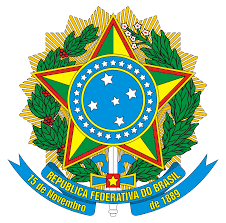
\includegraphics[width=2.5cm]{figuras/brasao-brasil}}
}{
%\Fonte{xxx}
}	
\end{figure}
\vspace*{-0.8cm}
\textbf{
SERVIÇO PÚBLICO FEDERAL \\
INSTITUTO FEDERAL DE EDUCAÇÃO, CIÊNCIA E TECNOLOGIA DO CEARÁ \\
CONSELHO SUPERIOR
}
\end{center}

\begin{center}
\textbf{RESOLUÇÃO N° 01, DE 10 DE JANEIRO DE 2018}
\end{center}

\vspace*{-1cm}

\begin{SingleSpace}
\begin{flushright}
\begin{minipage}[b]{8cm}
\begin{small}
Aprova \textit{ad referendum} a criação do curso Superior de Tecnologia em Gestão Ambiental no \textit{campus} Paracuru. 
\end{small}
\end{minipage}
\end{flushright}
\end{SingleSpace}

\textbf{O PRESIDENTE EM EXERCÍCIO DO CONSELHO SUPERIOR DO INSTITUTO FEDERAL DE EDUCAÇÃO, CIÊNCIA E TECNOLOGIA DO CEARÁ}, no uso de suas atribuições legais e estatutárias e considerando o Memorando n$^{\circ}$ 001/2018/GDG da direção-geral do campus Paracuru, 

\textbf{RESOLVE:}

\textbf{Art. $1^{\circ}$} - Criar, \textit{ad referendum} do Conselho Superior, o curso Superior de Tecnologia em Gestão Ambiental do \textit{campus} Paracuru e autorizar a oferta de 35 vagas semestrais.

\textbf{Parágrafo único} - O curso será ofertado na modalidade presencial e nos turnos matutino e vespertino, conforme definido no projeto pedagógico em anexo. 

\textbf{Art. $2^{\circ}$} - A interrupção da oferta e/ou a extinção do referido curso deverá ser submetida a este conselho para aprovação, com as devidas justificativas e a apresentação do planejamento de realocação de recursos humanos e de materiais vinculados ao curso.

\begin{center}
José Wally Mendonça Menezes \\
\textbf{Presidente em exercício do Conselho Superior}
\end{center}
%\imprimirindice

\end{document}
